\section{Einleitung}
Um das Verhalten von Mobilgeräten aufzuzeichnen, muss ein Versuchsumfeld 
geschaffen werden, welches erlaubt, die Geräte unter möglichst realitätsnahen 
Bedingungen zu messen.
Weiterhin soll das Versuchsumfeld verhindern, dass Störfaktoren die Messergebnisse 
beeinflussen.

Die beiden Anforderungen Wirklichkeitstreue und Störfaktorfreiheit schliessen
sich zum Teil gegenseitig aus.
Zum einen kann in einem isolierten Messraum nicht das selbe Umfeld simuliert 
werden, welches ein Mobilgerät im täglichen Gebrauch antrifft.
Zum anderen können Probe-Requests von anderen Geräten die Messergebnisse 
erheblich verfälschen, vor allem wenn diese Probe-Requests mit anonymisierten
MAC-Adressen durchgeführt werden und das zu messende Gerät nicht von den 
störenden Geräten unterschieden werden kann.

Es wurde entschieden, die Messungen in einem Faraday-Käfig 
durchzuführen, damit Fremdgeräte nicht die Versuche beeinflussen.
Das Institut für Kommunikationstechnik ICOM hat eine Antennenmesskammer 
für die Messungen von Antennen und Kommunikationssystemen.
Diese Messkammer kann Signale von ausserhalb des Messraums genügend abschirmen,
dass diese nicht die Elektronik im Messraum beeinflussen.
Nach einer kurzen Recherche wurde an Marcel Kluser verwiesen, 
der den Gebrauch der Messkammer für die Dauer der Experimente bewilligt hat.

\subsection{Versuchsaufbau}
Die Messkammer besteht aus einem Innenraum mit $1.5m$ x $2.5m$ Grundfläche, 
ist ca. $2m$ hoch und in der Kammer mit Schaumstoffspitzen ausgekleidet, 
welche die Signalausbreitung aus der Kammer eindämmen. 
Die Aussenhülle besteht aus Metall und kann durch eine Türe den Innenraum
komplett von der Aussenwelt abschotten.

In der Messkammer sind jeweils folgende Geräte im Betrieb:
\begin{itemize}
    \item Das zu messende Mobilgerät
    \item Ein Laptop mit Wireshark im Monitormodus oder ein WLAN-Messgerät, 
    angeschlossen an einen Laptop.
    \item Ein weiteres Mobilgerät für die Simulation eines WLAN-Access-Points.
\end{itemize}

Die Abbildung~\ref{figure:experimentalsetup} zeigt den Versuchsaufbau mit 
den verwendeten Geräten.

\begin{figure}[h!]
	\centering
	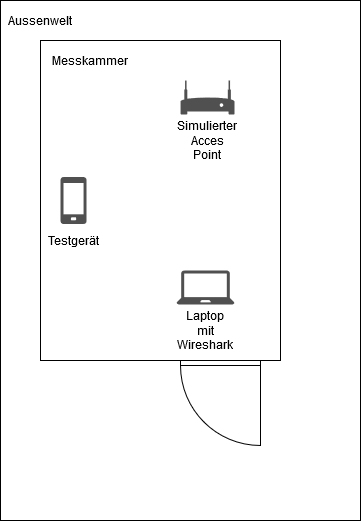
\includegraphics[width=1\linewidth]{Experiments/Messaufbau.png}
    \caption{Messaufbau in der Antennenmesskammer.
	\label{figure:experimentalsetup}}
\end{figure}

\clearpage

\subsection{Verwendete Tools}
Für die Versuchsdurchführung wurde ein Macbook verwendet, welches über eine 
Netzwerkkarte verfügt, die das Messen von Probe-Requests ermöglicht.
Auf dem Macbook ist Wireshark installiert, ein Netzwerk-Protokoll-Analyse-tool
welches die Analyse von Computersignalen verschiedener Protokolle erlaubt.
Der Monitormodus in Wireshark wird verwendet, um WLAN-Kommunikation im 
Empfangsbereich des Macbooks aufzuzeichnen.
Solange das Macbook Wireshark im Monitormodus betreibt, werden keine eigenen
Probe-Requests ausgesendet.
Weiterhin wurde ein WaveXpert WLAN-Messgerät verwendet, 
welches über einen Laptop betrieben wird und auf mehreren Kanälen gleichzeitig
Wireless-Kommunikation aufzeichnen kann.
Bei der Verwendung des WaveXpert werden die Probe-Request des Betriebslaptops
mit aufgezeichnet und müssen bei der Auswertung der Messergebnisse durch 
Filterregeln im Wireshark entfernt werden. 

Mit Wireshark aufgezeichnete Messungen werden als .pcapng-Dateien gespeichert,
welche mit Wireshark wieder geöffnet und analysiert werden können.
Es ist möglich, die Messungen in diversen Formaten zu exportieren, 
wobei das JSON-Format die ursprünglichen Informationen der Messung am 
besten erhält und Informationen in einer hierarchischen Struktur speichert,
die es erlaubt, die Messdaten einfach weiter zu verarbeiten.

Es wurde ein Python-Skript geschrieben, welches die Messdaten aus dem 
JSON-Format extrahiert und in ein Excel einträgt. 
Excel wurde für die Analyse ausgewählt, da in Excel sehr schnell einfache
Auswertungen durchgeführt werden können. 
Für die Weiterverarbeitung in einem Prototyp können die Daten in ein dafür
geeignetes Format codiert werden indem das Skript angepasst wird.

Um einen Access Point zu simulieren, wird ein weiteres Mobilgerät verwendet, 
welches in den dafür vorgesehenen Messungen einen Hotspot generiert.
Während den Messungen, die keinen Hotspot benötigen, befindet sich das
Mobilgerät im Flugmodus, um selbst keine Probe-Requests auszusenden.
Als zusätzliche Sicherheit wurde die Randomisierung von MAC-Adressen auf 
dem Mobilgerät ausgeschaltet, damit fälschlich ausgesendete Probes einfach
durch Filter entfernt werden können.

Die zu testenden Mobilgeräte werden in den jeweiligen 
Unterabschnitten genauer beschrieben.

\clearpage

\subsection{Durchzuführende Messungen
\label{subsection:plannedexperiments}}
Um das Verhalten der Mobilgeräte in verschiedenen Situationen aufzuzeichnen,
wurden diverse Tests spezifiziert.

Da die Mobilgeräte gemäss der Recherchen ein unterschiedliches Verhalten haben,
je nachdem ob sie in Gebrauch oder im Ruhemodus sind, werden die Tests in beiden
Zuständen durchgeführt.

Es soll gemessen werden, ob Geräte Probes aussenden, wenn die Wireless-
Einstellung ausgeschaltet ist. 
Da es möglich ist, dass dieses Verhalten in den Einstellungen angepasst werden
kann, müssen die Messungen jeweils mit den Einstellungen ein- und ausgeschaltet
durchgeführt werden (falls vorhanden).

Falls die Verschleierung der MAC-Adressen eine Einstellung auf dem Gerät ist,
soll jeweils für beide Einstellungen eine Messung durchgeführt werden.

Da in früheren Arbeiten die Anzahl bekannter Access Points auf dem Mobilgerät
die Anzahl ausgesandter Probe-Request beeinflusst hat, sollen alle Messungen
mit unterschiedlicher Anzahl bekannter SSID's durchgeführt werden.

Damit das Probing-Verhalten eines Mobilgeräts während dem Einschalt-vorgang und
beim Wechsel in den bzw. aus dem Flugmodus aufgezeichnet werden kann, 
werden Messungen durchgeführt, während das Mobilgerät respektive der 
Flugmodus abwechslungsweise ein- und ausgeschaltet wird.

Weiterhin soll untersucht werden, ob Mobilgeräte, die mit einem Access Point
verbunden sind, weiterhin Probe-Requests aussenden und ob in diesen Frames 
die MAC-Adresse verschleiert ist.

Für den Betrieb im Ruhemodus, im aktiven Modus und mit verbundenem WLAN 
ist jeweils zusätzlich eine Langzeitmessung von einer Stunde vorgesehen, 
um genügend Frames aufzuzeichnen, dass ein mögliches Pattern in der 
Randomisierung der MAC-Adresse oder der Sequenznummer erkannt werden kann.
Die anderen Messungen sind auf ein Zeitfenster von zehn Minuten begrenzt, wobei
bei den Messungen mit ausgeschaltetem WLAN der Versuch abgebrochen wird, falls 
nach einer Minute keine Probe-Requests aufgezeichnet werden.

Gesamthaft werden pro Mobilgerät neun Stunden lang Messungen durchgeführt, 
wobei zwei Stunden und 40 Minuten eingespart werden können, wenn mit 
ausgeschaltetem WLAN keine Probe-Requests ausgesendet werden.

Zusätzlich sollen Messungen mit mehreren Mobilgeräten im Empfangsbereich
durchgeführt werden, um realistische Messdaten zu erhalten. 
Mit diesen Messungen kann ein  Prototyp während der Entwicklung verifiziert 
werden.  

\clearpage

\subsection{Erwartete Messergebnisse}
In der Recherche hat sich herausgestellt, dass moderne Betriebssysteme von 
Mobilgeräten die MAC-Adresse für sämtliche Probe-Requests randomisieren sollten, 
solange sie nicht mit einem Access Point assoziiert sind. 
Weiterhin sollten die Sequenznummern auch zufällig für jede Gruppe von 
Probe-Requests neu gesetzt werden.
Es wird davon ausgegangen, dass die herstellerspezifischen Felder in den Frames
der Probes nicht mitgesendet werden und die IE-Felder zwischen den Probe-
Requests von unterschiedlichen Geräten mehrheitlich identisch sind.

Die einzigen zwei Möglichkeiten, den Geräten einen Fingerprint zuzuweisen,
sehen die Autoren in der Reihenfolge und Anzahl der IE-Felder oder über einen 
Timing-basierten Ansatz.

\subsection{Messplan}
Die Tabellen~\ref{table:experimentalplanone} und~\ref{table:experimentalplantwo} 
zeigen die Messplanung, welche für die Versuche in der Messkammer verwendet 
wurde.

\begin{table}[h!]
	\centering
	\begin{tabular}{|c|c|c|c|c|}
		\hline
        \textbf{Testbeschreibung} & \textbf{WiFi} & \textbf{Privacy-Settings} & \textbf{Zeit}  \\
        \hline
        Messung im Startup & Ein & Ein & 10 min  \\
        Mit WLAN verbunden & Ein & Ein & 10 min  \\
        Suche nach versteckter SSID & Ein & Ein & 10 min \\
        Messung im Flugmodus & Ein & Ein & 10 min \\
        \hline
        Langzeitmessung Ruhemodus & Ein & Ein & 60 min \\
        Langzeitmessung Aktivmodus & Ein & Ein & 60 min \\
        Langzeitmessung Verbunden & Ein & Ein & 60 min \\
        \hline
    \end{tabular}
    \caption{Messplan: SSID-unabhängige Messungen
    \label{table:experimentalplanone}}  
\end{table}

\begin{table}[h!]
	\centering
	\begin{tabular}{|c|c|c|c|c|c|}
		\hline
        \textbf{Testbeschreibung} & \textbf{WiFi} & \textbf{Privacy-Settings} & \textbf{Zeit} & \textbf{Bekannte SSID's} \\
        \hline
        Gerät im Ruhemodus & Ein & Ein & 10 min & 10 \\
        & Ein & Aus & 10 min & \\
        & Aus & Ein & 10 min & \\
        & Aus & Aus & 10 min & \\ 
        Gerät aktiv & Ein & Ein & 10 min & \\
        & Ein & Aus & 10 min & \\
        & Aus & Ein & 10 min & \\
        & Aus & Aus & 10 min & \\ 
        \hline 
        Gerät im Ruhemodus & Ein & Ein & 10 min & 5 \\
        & Ein & Aus & 10 min & \\
        & Aus & Ein & 10 min & \\
        & Aus & Aus & 10 min & \\ 
        Gerät aktiv & Ein & Ein & 10 min & \\
        & Ein & Aus & 10 min & \\
        & Aus & Ein & 10 min & \\
        & Aus & Aus & 10 min & \\
        \hline 
        Gerät im Ruhemodus & Ein & Ein & 10 min & 1 \\
        & Ein & Aus & 10 min & \\
        & Aus & Ein & 10 min & \\
        & Aus & Aus & 10 min & \\ 
        Gerät aktiv & Ein & Ein & 10 min & \\
        & Ein & Aus & 10 min & \\
        & Aus & Ein & 10 min & \\
        & Aus & Aus & 10 min & \\  
        \hline 
        Gerät im Ruhemodus & Ein & Ein & 10 min & 0 \\
        & Ein & Aus & 10 min & \\
        & Aus & Ein & 10 min & \\
        & Aus & Aus & 10 min & \\ 
        Gerät aktiv & Ein & Ein & 10 min & \\
        & Ein & Aus & 10 min & \\
        & Aus & Ein & 10 min & \\
        & Aus & Aus & 10 min & \\ 
        \hline
    \end{tabular}
    \caption{Messplan: SSID-abhängige Messungen
    \label{table:experimentalplantwo}}  
\end{table}

\clearpage

\subsection{Beschaffung der Geräte}
Um an Mobilgeräte für die Messungen zu kommen, wurden verschiedene mögliche 
Quellen angefragt.
Das Institut für Softwareentwicklung IFS unterhält mehrere Mobilgeräte für 
Test-, Entwicklungs- und Ausstellungszwecke, die für die Versuche ausgeliehen
werden durften.
Weiterhin wurde im Freundes- und Familienkreis nachgefragt, 
ob moderne Mobilgeräte mit den zu messenden Betriebssystemversionen 
verwendet werden und ob diese ausgeliehen werden dürfen.
Es hat sich herausgestellt, dass iPhones im persönlichen Umfeld weniger in 
Gebrauch sind als Android-Geräte.
Dies stellt allerdings kein grösseres Problem dar, 
da Android auf einem breiteren Spektrum von Hardware verwendet wird, 
die potentiell grösseren hardwarespezifische Abweichungen im Verhalten aufweisen können.

Welche Mobilgeräte tatsächlich für die Messungen verwendet wurde, 
wird in den jeweiligen Abschnitten beschrieben.

\clearpage